\end{multicols}
 \mysection{Medicine}{vulgate-medicine}

  \callout {
    \begin{center}
    You can only practice Medicine during \mylink{Downtime}{downtime}.
    \end{center}
}


 \mylink{Beatings}{physical-wound-beating}, \mylink{Addiction}{gear-narcotics-addiction}, and \mylink{Disease}{vulgate-medicine-diseases} need the careful ministrations of a medic and a period of convalescence before an Adventurer returns to full strength. The Vulgate of Medicine teaches the herbs, minor incantations, odd pharmaceuticals, weird bloodletting practices, etc. required to bring someone back from their brush with death.

Medicine can only be practiced in the \mylink{Shopping Step}{downtime-shopping} during \mylink{Downtime}{downtime}. Each Beating, Addiction, or Disease you remove through rehabilitation \mybold{will cost you 100\AG in supplies}. See the section on \mylink{Downtime}{downtime} for more information.

The Vulgate of Medicine cannot remove \mylink{Madness!}{injury-insanity-madness}; the injuries of the mind require either a visit to a \mylink{Chirurgeon}{gear-services}, or a dose of \mylink{Laudanum}{research-chymistry-laudanum}.


\callout {
    If you are receiving Medicine through the ministrations of a \mylink{Chirurgeon}{gear-services}, multiply the costs by 5x (so 500\AG).
}

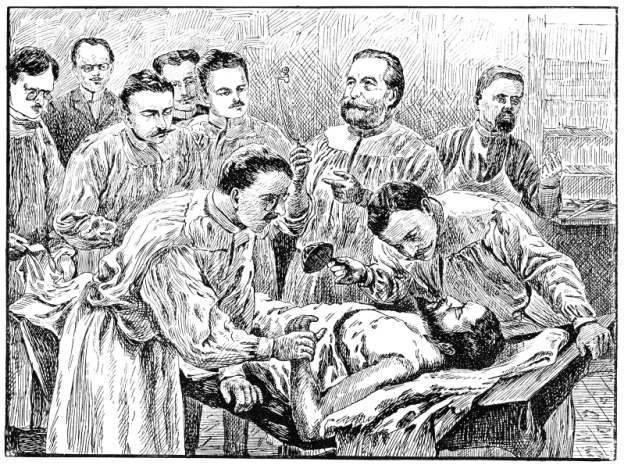
\includegraphics[width=\columnwidth]{vulgate/Medicine}

\newpage

\crunch{A Spoonful Of...}{vulgate-medicine-crunch}

You can optionally make the cure a \mylink{Side Story}{downtime-side-story} by using Logan Knight's delightful \href{https://www.lastgaspgrimoire.com/does-this-look-infected/}{Does This Look Infected?}, or create your own. I've included 12 of my favorites below.


  \mytable{l X} {  
  } {

    1 &  While breathing in the fragrant smoke of burning Govora pollen, ingest a pint of pig urine to induce vomiting. Drown a nightingale in the spilled contents of your stomach within the waiting iron urn, then keep the drowned body beneath your bed for three days before throwing it out the East window. \\
    2 &  A pregnant rat, teeth pulled and pups moving beneath fat-smeared fur, must be swallowed alive. When it gives birth to its young the affliction will pass onto them before they die and pass through your digestion.\\
    3 &  Your face must be smothered with a duck-down pillow soaked in vinegar and hyena urine. When you finally struggle for breath at the point of collapse the pillow will be removed so that you may be slapped full in the face with a stillborn hound. This will be repeated as many times as necessary. \\
    4 &  Hold six blessed sparrow eggs in your mouth and descend into the Corpusmilch Canal, do not swallow them until you touch the bottom.\\
    5 &  Your body will be smeared with the putrescent black mud of the Nameless Bog. Ingest a small amount, be cautious not to consume too much, and do not bathe until two days have passed.\\
    6 &  Submerge yourself in a copper bath of goat's milk while suckling at the teat of a wetnurse until the malady has passed.\\
    7 &  Swallow a river stone wrapped in maiden's hair. The hair will absorb the affliction and pass from you along with the stone. \\
    8 &  The affliction must be drawn out through the skin. Cupping using the severed horns of a tribe of black goats sacrificed beneath the full moon will relieve the malady. \\
    9 &  The afflicted area must be wrapped in dried kelp that was once soaked in the urine of an unfaithful man. The smoldering ashes of a sapling will then be laid upon it until they have burnt through and touched flesh. \\
    10 & Inhale a pinch of blue moss from the silver-gilded goat's head snuff mull and seek the Divine Polycerate Goat in your dream wanderings. Supplicate before him and he may gnaw the affliction from your being. \\
    11 & A candle made from the fat of a drowned man and scented with Spring's first bloom must be sat upon the forehead and allowed to burn down to hard streams of yellow nothing. \\
    12 & You must lie within a circle of blessed yellowed candles, with the ashy pollen of the Widow's Blossom dusted upon your face. Throughout the night the affliction will call to you from beyond the waxen circle in voices myriad and sweet. If you resist their call until morning, it will pass. \\
}

\newpage

\mysubsection{Diseases}{vulgate-medicine-diseases}

Just before the end of each Session, anyone who has come Close to the infected must \RSTRY{\VIG}; if they fail, they become infected with the disease as well.

A handful of Diseases worsen over a number of Sessions.  Wherever that's mentioned, it needs to be cured by the end of the Session indicated i.e.  if it says "after 4 Sessions, you suffocate", that means you have until the end of the 4th Session to get treatment, or ... you know, suffocate.  Receiving a cure reverses all the effects of the Disease unless they are permanent.

Here are 16 various diseases converted to ToY rules, using Logan Knight's \href{https://www.lastgaspgrimoire.com/does-this-look-infected/}{Does This Look Infected?} to get you started; you should definitely make your own.


  \mytable{l X} {  
  } {
    1 &  Your skin grows raw and red and sprouts enormous blood blisters that swell to the size of a small apple before popping in arcs of putrid plasma, over and over again like boiling mud baths. You can't wear any clothing, let alone Armor. \\
    2 &  Pus weeps from your throat and crusts into barnacle-like lesions on your neck, causing intense pain if you speak anything but lies.  \\
    3 &  A crater-like pox mars the flesh around the wound and creeps up your neck. The vinegary stench grows when you are under stress or heightened excitement and puffs of yellow vapor vent from the pox. \SAVE{Toxins}whenever you enter Combat or do something strenuous.  If you fail, you are Befuddled for \DUR{d8}. \\
    4 &  The wound will not heal properly; rather than closing, small bunches of fleshy tendrils emerge from the cloven flesh, like the fingers of babies.  You are unable to restore Grit. \\
    5 &  Thick black tears leak from your eyes, clouding your vision, and you find that after you have wiped them away, when your fingers are stained black with oil, your eyelids cling together every time you blink, your hands stiffen, like fingertrap lockjaw.  You are permanently \mylink{Blind}{effect-blinded} within Days.  \\
    6 &  The skin around the wound hardens and crusts in blackening shards like a burning tree, then begins its creeping spread. You have extra Armor of \UDD{d4} for two Sessions - after that, your joints begin to stiffen, walking becomes a chore, you'd rather lay down in the dirt, bury your fingers and breathe in the muck. Every Session afterwards your \MD drops \DCDOWN.  If your \MD becomes \mylink{Spent}{dice-spent}, you become a tree permanently.  \\
    7 &  Your organs grind and groan like a wounded animal. You spend every Bivouac in agony while you pass a grotesque opalescent kidney stone. You are unable to heal Grit during this time.  A Philosopher could use this stone as a \mylink{Component}{arcana-wizardry-components}.  \\
    8 &  Every Combat, \RSTRY{\VIG}.  On a Failure you disgorge a surging mass of green bile that continues to bubble and churn after it has left your throat.  This incapacitates you for the rest of the fight.  \\
    9 &  Gob Rot. Your gums fester and peel back, you swallow parts of your tongue as it begins to putrefy, teeth drool out of your mouth while you speak.  After 4 Sessions, you permanently lose your ability to speak.  \\
}  

\mytable{l X} {
} {
    10 &  Swollen boils sprout from your skin, oddly puckered like an anus. After the 3rd Session, the next time you are amongst a large group of people they unfurl like glistening mucus-coated blossoms of skin, violently jettisoning flesh spores into the air.  Everyone Close to you is automatically infected with the disease (no Save).  The explosion doesn't kill you - the cycle now repeats itself. \\
    11 &  Fibrous purple fronds curl out from your skin, interwoven and fragile, ever-growing. It would be beautiful if they weren't siphoning off your blood supply.  At the start of the next Session, lose 1 \MAX Flesh.  At the start of the second Session lose 2 \MAX Flesh, etc.  When you hit 0 Flesh, you die.  \\
    12 &  The flesh around the wound becomes spongy, pliant, it exudes the scent of fuchsia. Synaesthesia ravages your psyche, and pulling away clumps of your deteriorating body makes the most deliriously beautiful music.  You are overcome and essentially \mylink{Paralyzed}{effect-paralyzed} (your friends can carry you).  If you are not cured within 2 Sessions, the effect is permanent.  \\
    13 &  Your flesh sloughs, a bicep one moment and a sack of atrophied muscle hanging from bone in a skin bag the next. But that's not what bothers you, it's when it comes back. Creeping up the bone, tendons attaching, muscle re-adhering, the sucking sounds within your skin. It never rebuilds the same way and your skin is starting to smell of rot.  Happens once every Session; whenever it happens, your \MAX:\VIG moves \DCDOWN.  If your \VIG ever becomes \mylink{Spent}{dice-spent} you die.  \\
    14 &  Your skin is pocked with holes like the back of a pregnant frog. Fleshy nodules emerge to squirt thin streams of noxious green fluid before retreating back inside your skin. It isn't an infestation, it is your own flesh, and it is growing larger.  After 3 Sessions, you explode in a massive blast of acidic green bile at a time that is most amusing to the Arbiter. Everyone Close to you is automatically infected with the disease (no Save).  The explosion kills you.  \\
    15 &  Resinous Influenza. It's not the bleary leaking eyes that bother you, nor the deep-bone ache or even the delirious shakes. It's the absurd amount of mucus that you expel every time you sneeze and the fact that it sets like resin almost as soon as it touches your exposed skin. Your face begins to look like a grotesque melted mask and that is not a good look for anyone.  You can't chip the mucous off.  You begin asphyxiating in your own mucous.  After 2 Sessions you will start having difficulty breathing; after 4 Sessions, you suffocate. \\
    16 &  Polychromous Decay. It starts with a dry itch, dustings of dead flakes falling from your skin as you scratch like chronic dandruff, turning strangely polychromatic as it settles. After Hours the disease makes its way into your flesh, and your skin has almost entirely itched away and you're scratching canals into the muscle beneath. It doesn't even look like flesh and blood anymore, just polychromatic granularity like a bathbomb.  After 2 Sessions your hands have been ground away so you rub your itching limbs together as best you can, grinding biceps over your torso, crushing your chin against your chest.  Finally, after 4 Sessions, without anything left to scratch it with, you find that your flesh slowly regrows, but the moment your limbs build back into movable stumps... The Polychromous Decay is a powerful spell component and many of those who contract its disease end up as limbless torsos in a Philosopher's basement, unable to scream through dust-filled lungs, forever regenerating porous dusty flesh only to have it scraped away.  \\
}

